
\documentclass[12pt]{amsart}
\usepackage{listings}
\usepackage{color}
\usepackage{graphicx}

\definecolor{dkgreen}{rgb}{0,0.6,0}
\definecolor{gray}{rgb}{0.5,0.5,0.5}
\definecolor{mauve}{rgb}{0.58,0,0.82}

\lstset{frame=tb,
  language=Python,
  aboveskip=3mm,
  belowskip=3mm,
  showstringspaces=false,
  columns=flexible,
  basicstyle={\small\ttfamily},
  numbers=none,
  numberstyle=\tiny\color{gray},
  keywordstyle=\color{blue},
  commentstyle=\color{dkgreen},
  stringstyle=\color{mauve},
  breaklines=true,
  breakatwhitespace=true,
  tabsize=3
}
\title{NLP_HW3}
\author{Xuan Wang}
\date{} % delete this line to display the current date

%%% BEGIN DOCUMENT

\begin{document}
\begin{titlepage}

\begin{center}


% Upper part of the page

\textsc{\LARGE University of Rutgers}\\[1.5cm]

\textsc{\Large Assignment 1: Fast Trajectory Planning}\\[0.5cm]


% Author and supervisor
\begin{minipage}{0.4\textwidth}
\begin{flushleft} \large
\emph{Author:}\\
Xuan \textsc{Wang}

Xunjie \textsc{Zhu}
\end{flushleft}
\end{minipage}
\begin{minipage}{0.4\textwidth}
\begin{flushright} \large
\emph{Supervisor:} \\
Abdeslam  \textsc{Boularias}
\end{flushright}
\end{minipage}

\vfill

% Bottom of the page
{\large \today}

\end{center}

\end{titlepage}

\section*{Part 0}
For the maze, define a maze class, use \emph{numpy} external library to generate a 2-d 101*101 int array representing the maze. Then use \emph{networkx} library to convert the maze into an undirected graph by adding edges for each pair of adjacency nodes, use \emph{dfs\_preorder\_nodes()} method to find a traverse list by DFS, for each visited node make it blocked of 30\% chance
\begin{lstlisting}
self.array = np.zeros((m,n))
traverselist = list(nx.dfs_preorder_nodes(self.graph,(0,0)))
p_list = [1,1,1,0,0,0,0,0,0,0]
traverselist = self.DFS()
for i in traverselist:
	self.array[i[0],i[1]] = random.choice(p_list)
\end{lstlisting}
The following picture is a visualization implement by scala


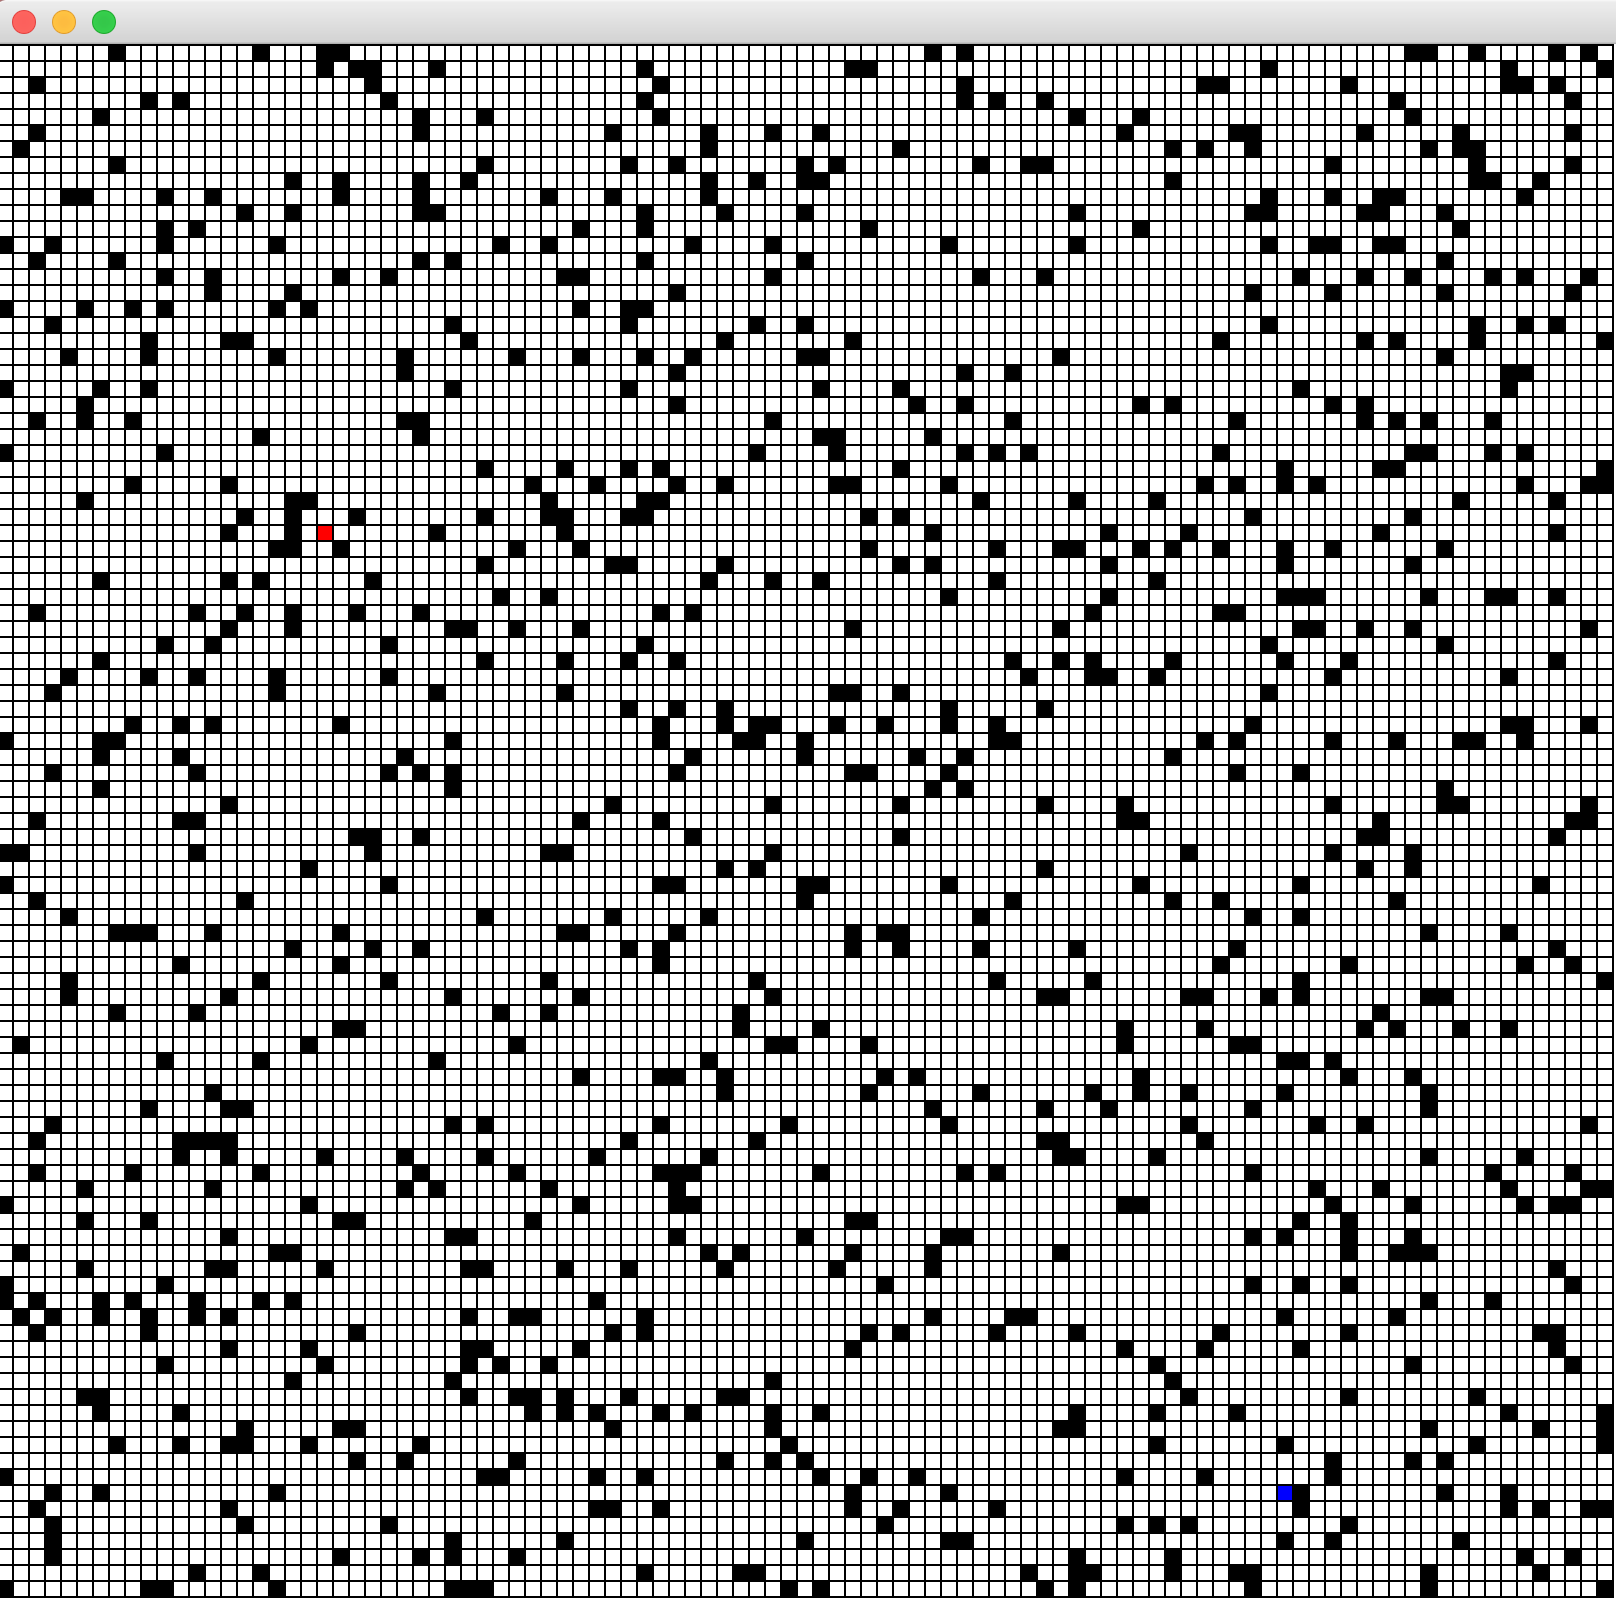
\includegraphics[width=1\linewidth]{maze.png}

\section*{Part 1}
(a)While the initial agent explored three cells next to it which is unblocked, the three cells have same \emph{g-values} 1, different \emph{h-values}. Base on Manhhatan distance, the right one cell has the samllest \emph{g-value} 2, so it has the smallest \emph{f-value} 3, so the right one will be expanded first.

(b)Since the algorithm finds cell with minimum f value from open list and add it to close list, if open list is running to empty without found a end node, that means no more unvisited cells can be expanded and there is no path from start node to target node. It is always possible to find a path or find it impossible before all unblocked cells are added into close list, so the result can be found in finite time. The worst case is that the agent finds block and change path at each unblocked cell, and for each cell the agent goes through all possible unblocked cells and find a dead end. So the bound of agent moves is the number of unblocked cells squared.

\newpage
\section*{Part 2}
Both version of Forward A* use the same generated maze to test, start point is in the upper left corner of maze, target point is in the lower right corner of maze and the following are the results:

(1) break ties in favor of small g value

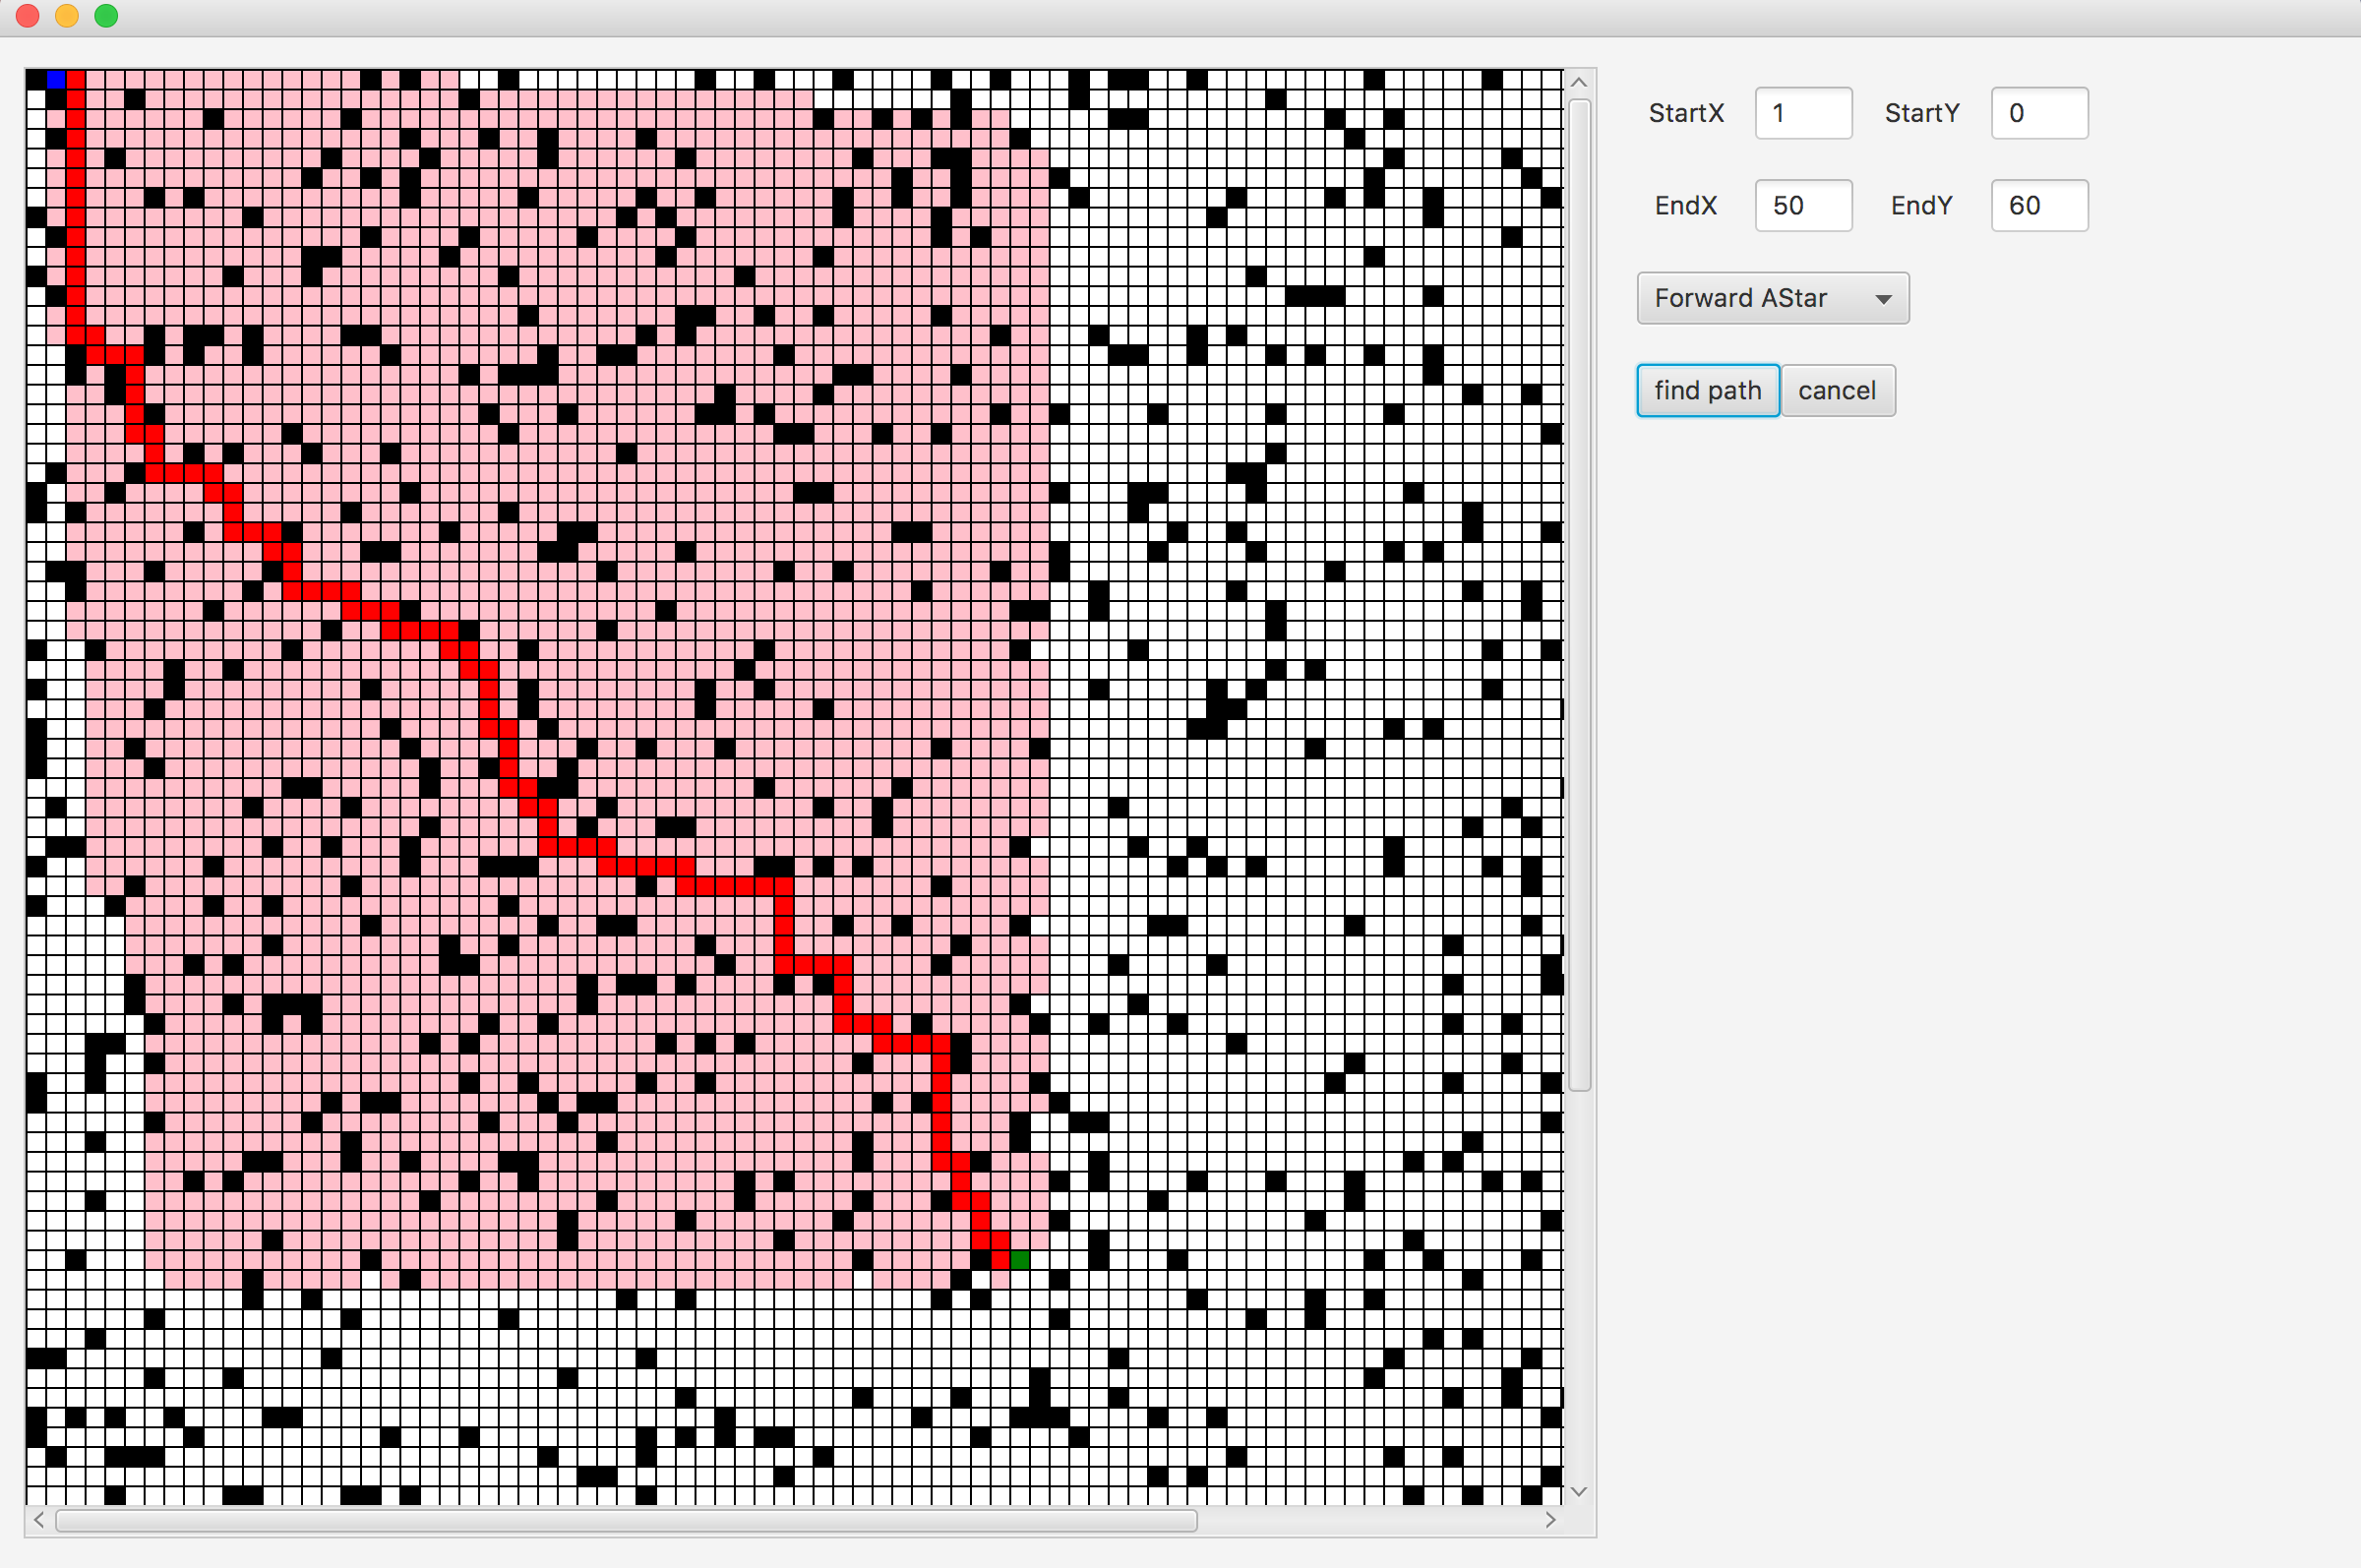
\includegraphics[width=1\linewidth,height=3in]{small_g.png}

(2) break ties in favor of larger g value

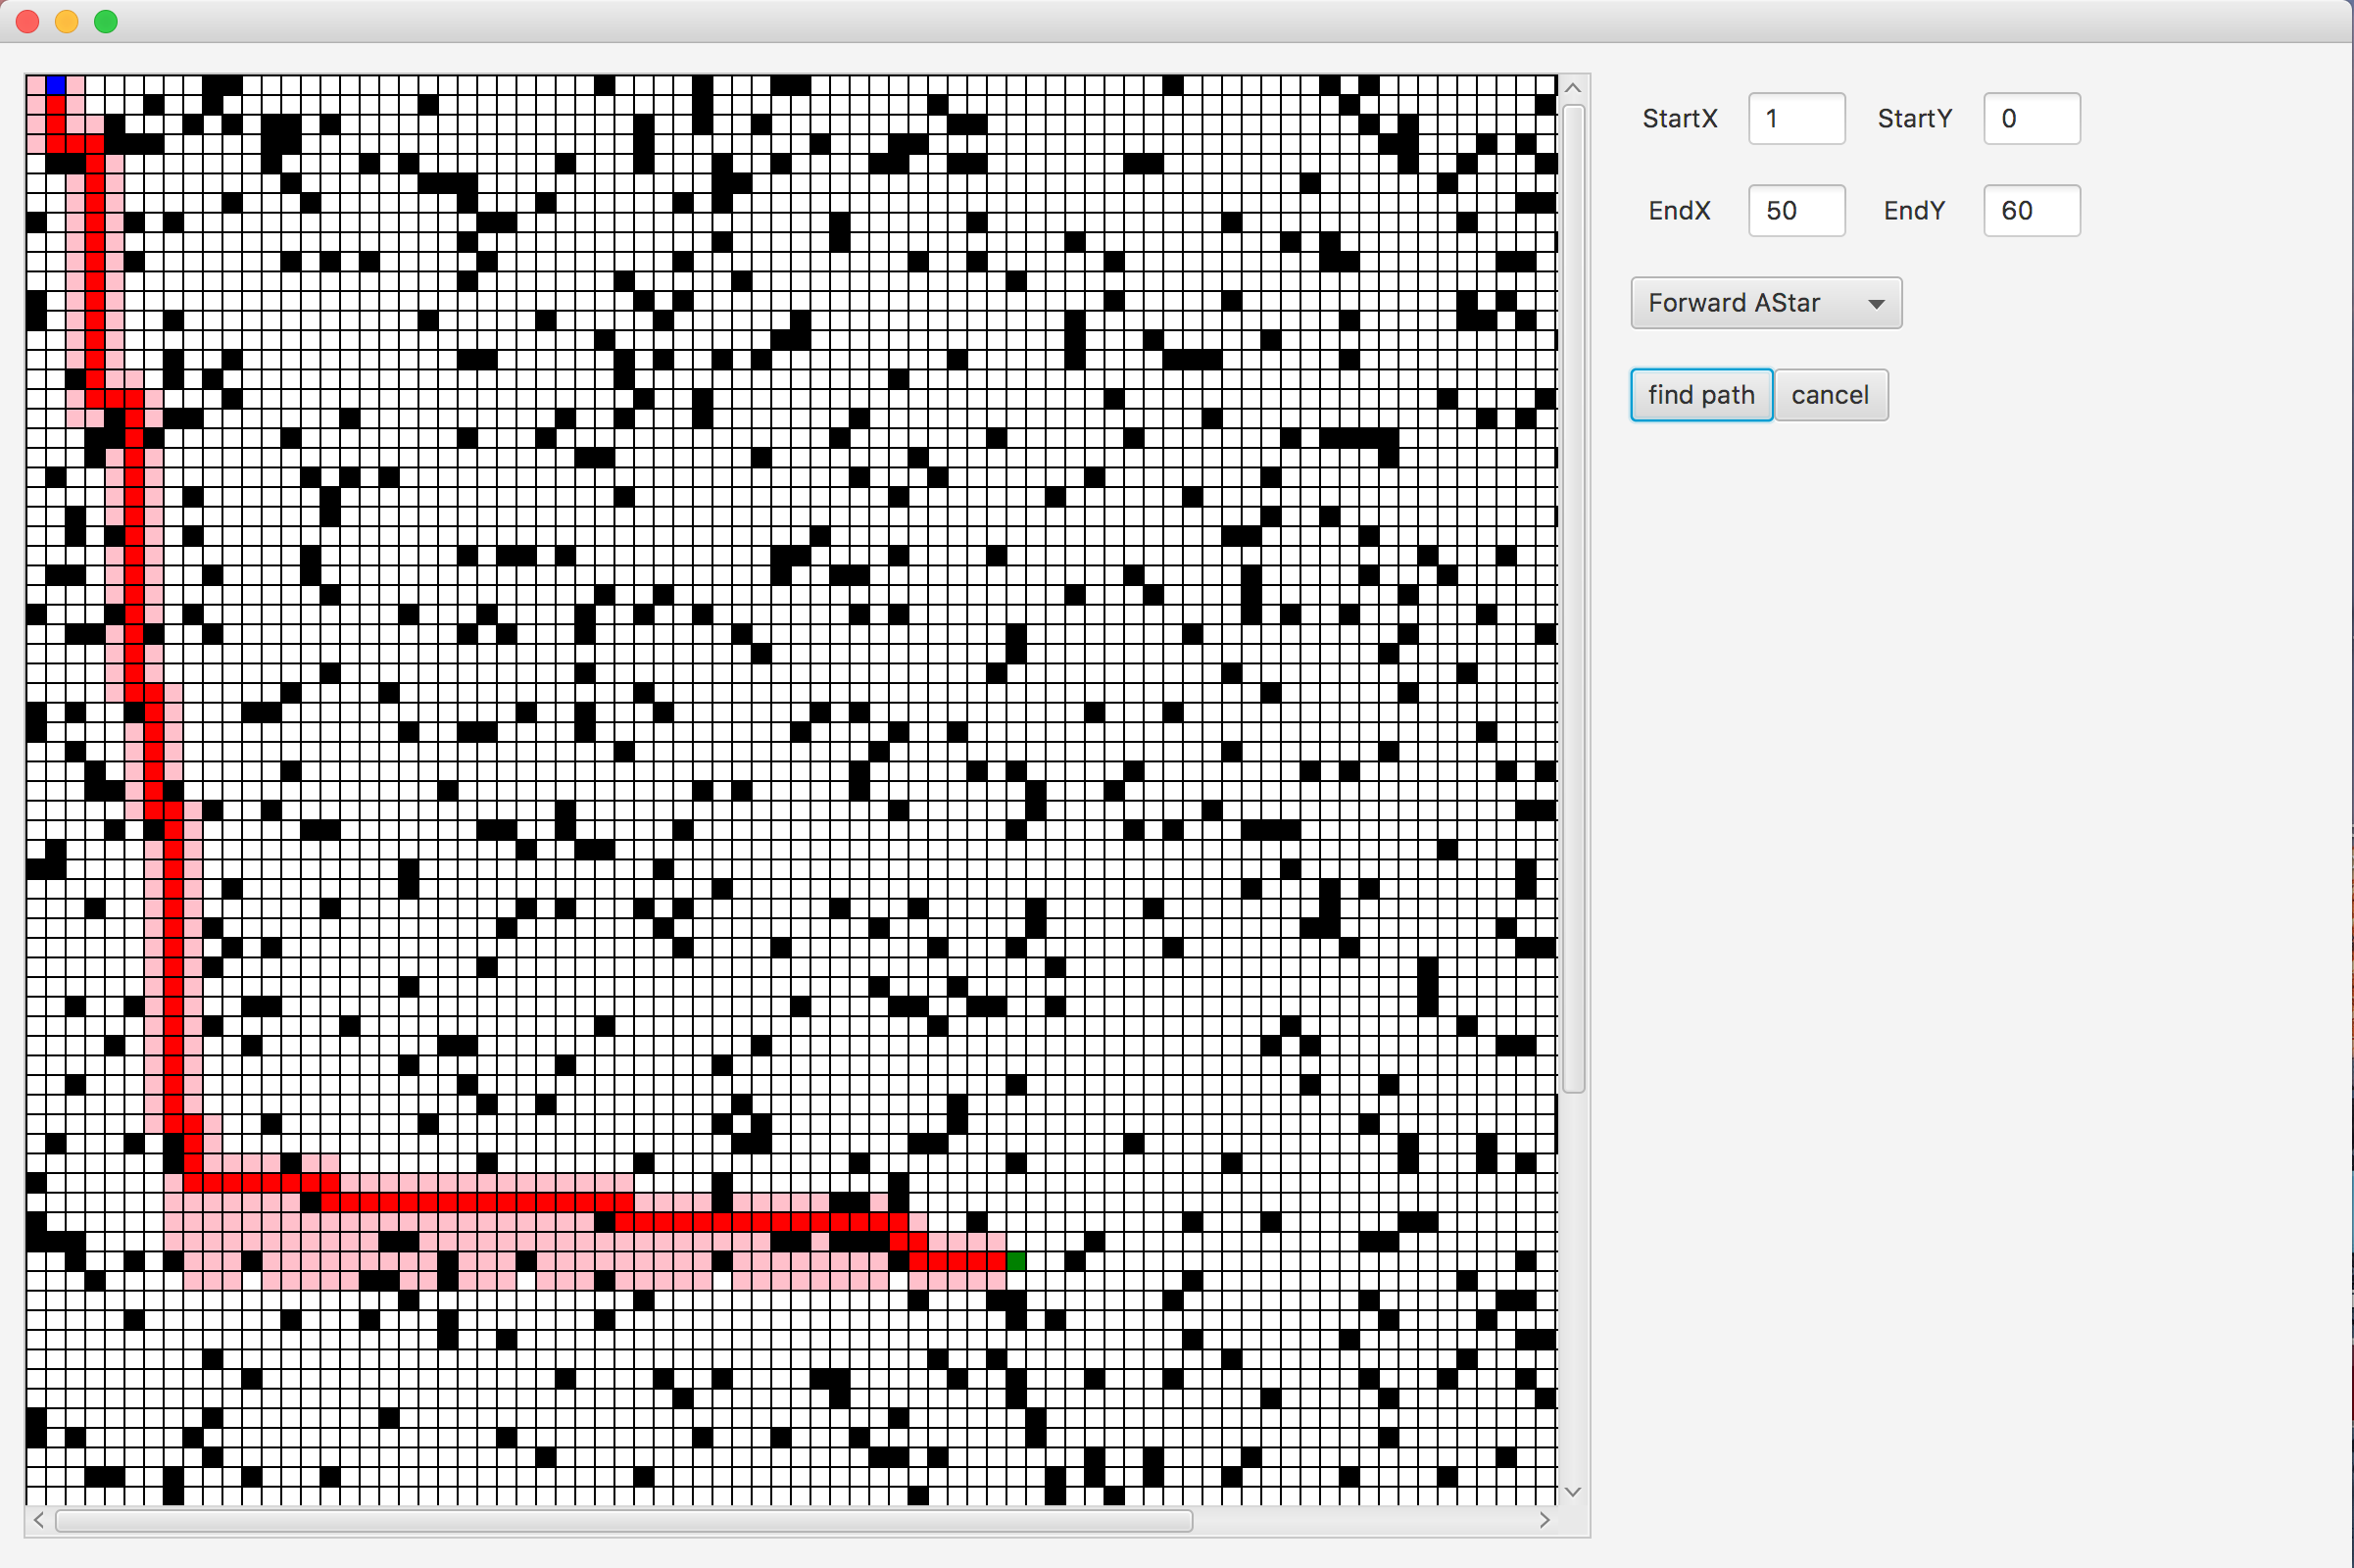
\includegraphics[width=1\linewidth,height=3in]{big_g.png}

cell with pink color in graphs means this cell is expanded and added to close list, apparently choosing small g value to break ties cause more cells be expanded than choosing larger g value. It is because the computer will always choose the farthest point away from the start point if a cell with larger g value has priority, and the search point will leave the start point as quickly as possible. If smaller g value is chosen, it is likely that cells having same f value around the start point will be searched level by level with the increasing of g value. \emph{A1 B1 C1 D1 E1 E2 E3 E4} cells will be expanded by both in Figure 9.
\newpage
\section*{Part 3}
\subsection*{3.1}
Repeated Forward A*

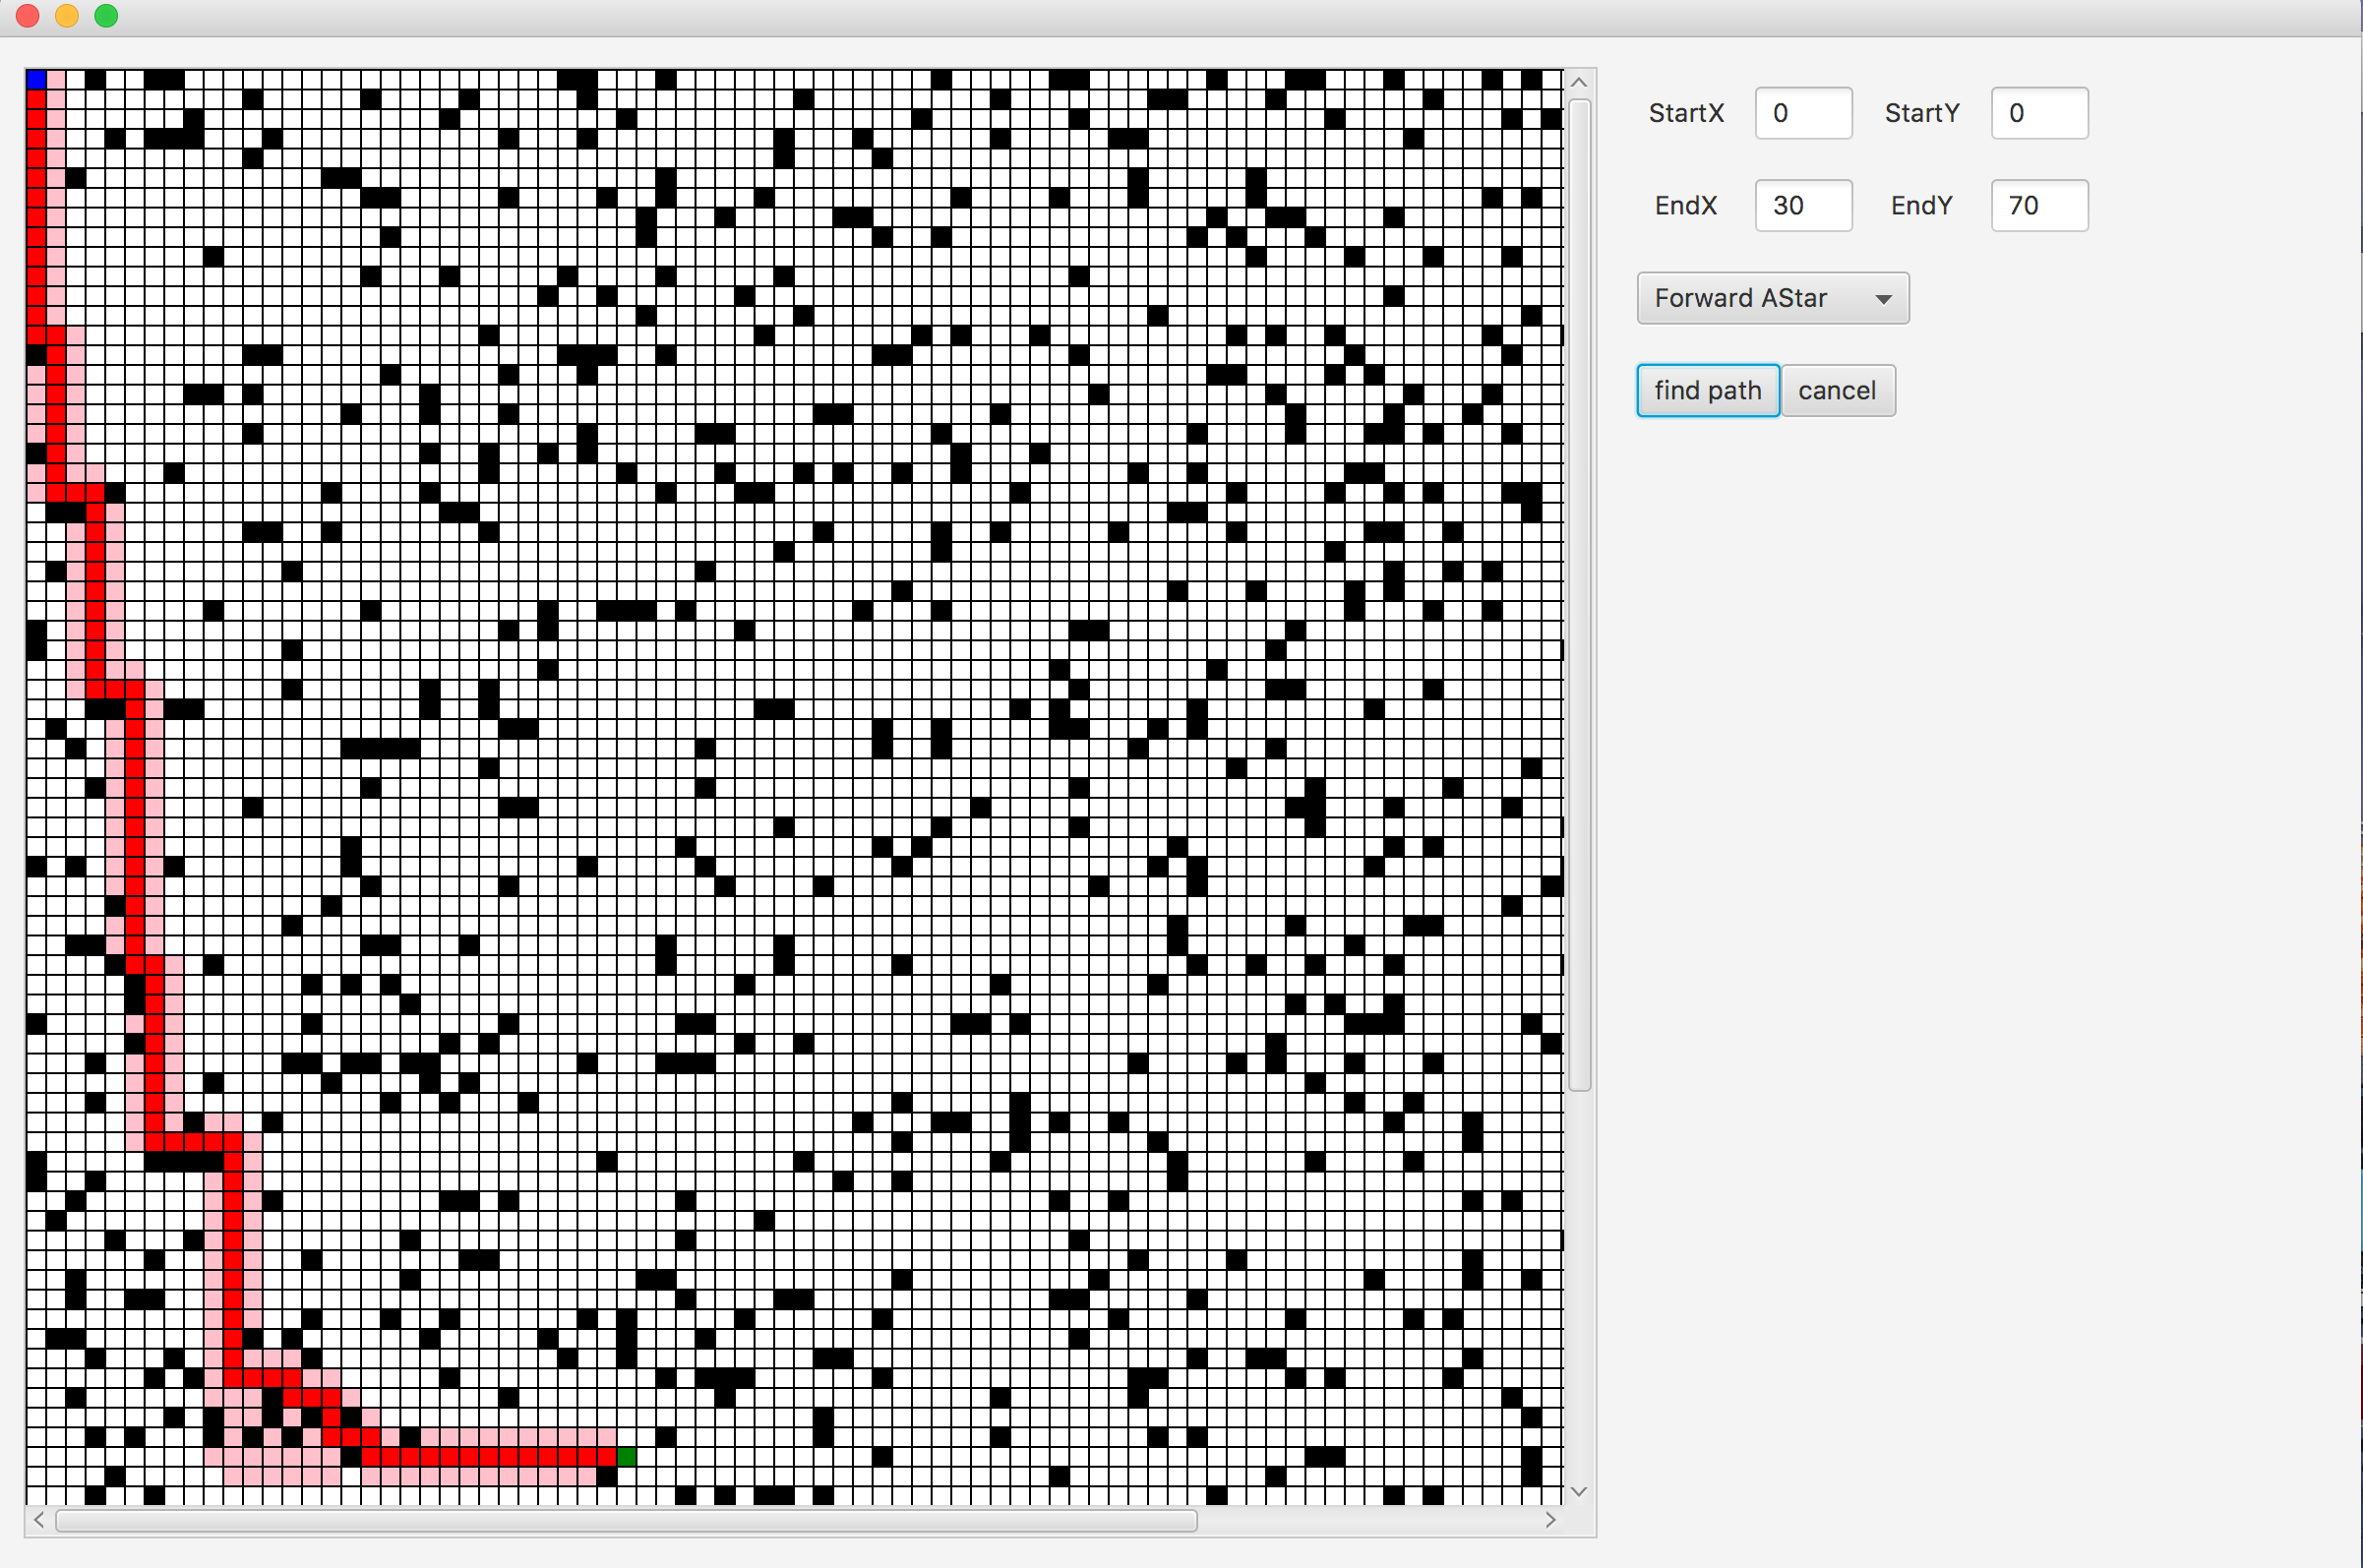
\includegraphics[width=1\linewidth,height=3in]{forward_30.png}

\subsection*{3.2}
Repeated Backward A*

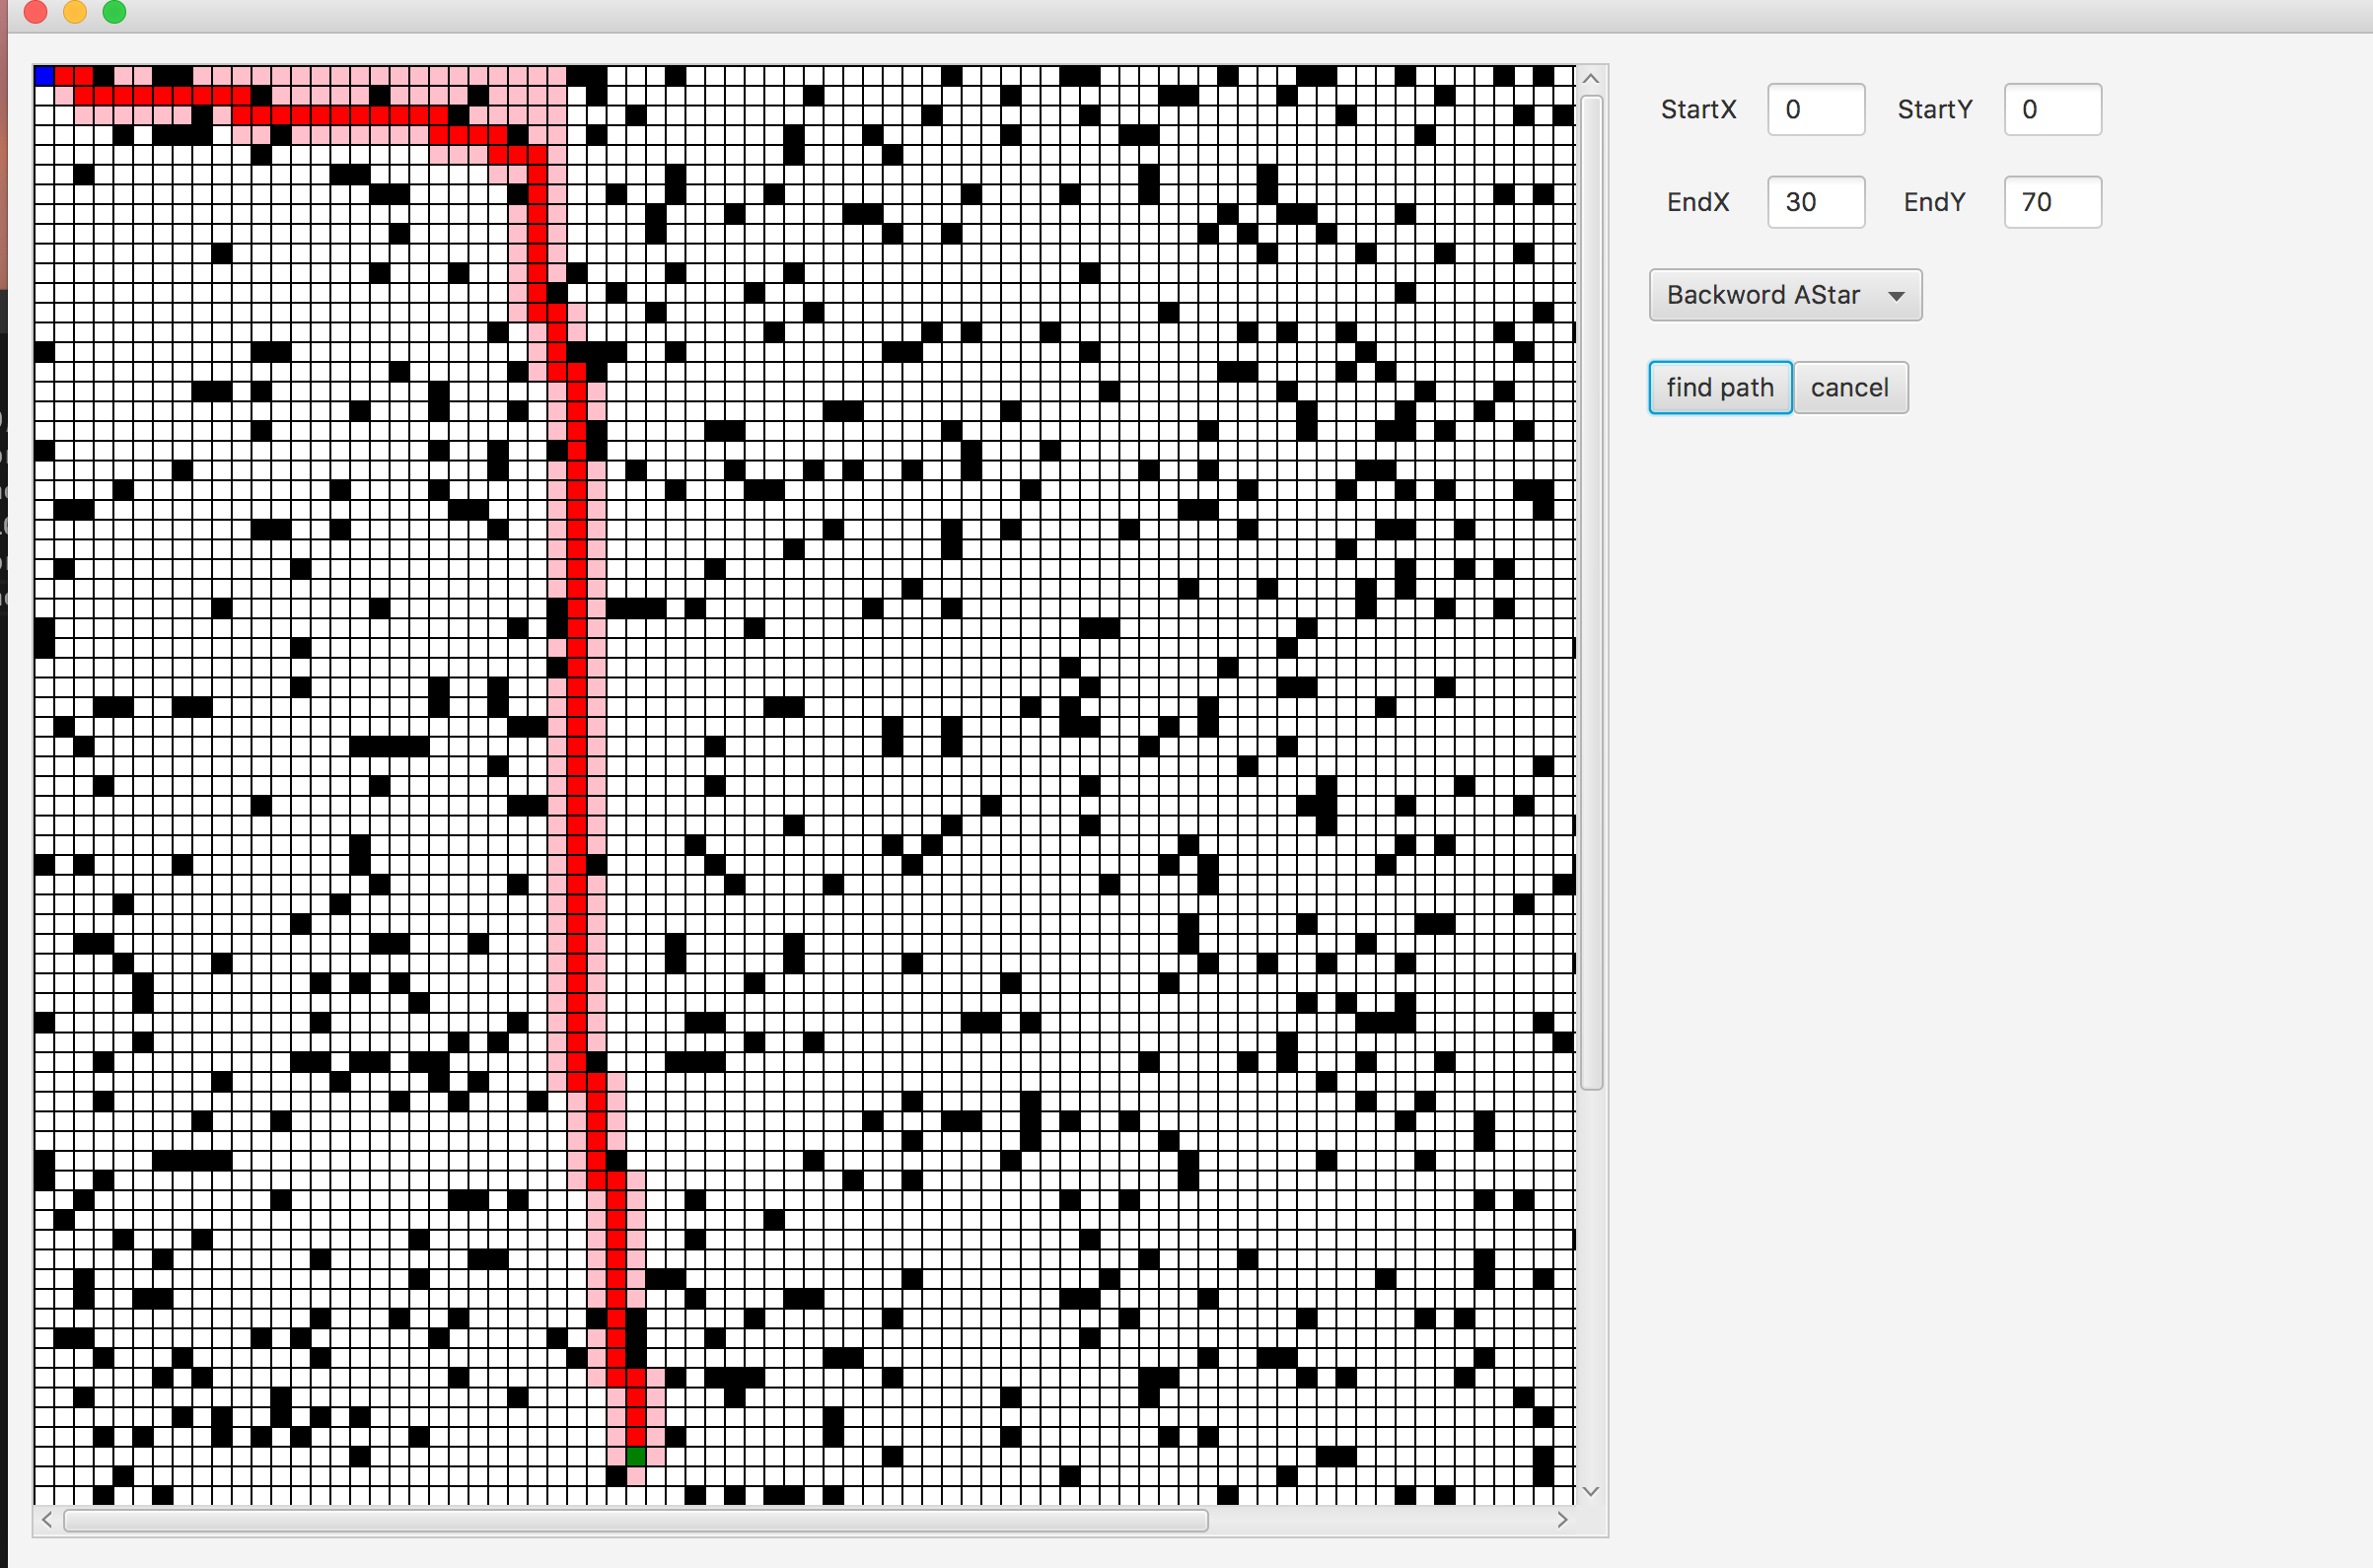
\includegraphics[width=1\linewidth,height=3in]{backward_30.png}

the results show that Repeated Forward A* and Repeated Backward A* have no significant difference, they have almost the same running time and same expanded number of cells and different paths. The cause of difference of paths is that they have the same break ties rule.
\section*{Part 4}
The definition of Manhattan distance: The distance between two points measured along axes at right angles. If the agent only moves in four compass directions, it will only move along the axes we built, it assures that the Manhattan distances are consistent.

(OFFICIAL ANSWER)Adaptive A* solves a series of similar but not necessar- ily identical search problems. However, it is important that the h-values remain consistent with respect to the goal state from search problem to search problem. The following changes can occur from search problem to search problem:
? The start state changes. In this case, Adaptive A* does not need to do anything since the h-values remain consistent with respect to the goal state.
? The goal state changes. In this case, Adaptive A* needs to correct the h-values. Assume that the goal state changes from sgoal to s?goal. Adaptive A* then updates (= overwrites) the h-values of all states s by assigning
h(s) := max(H (s, s?goal ), h(s) ? h(s?goal )). (2)
The updated h-values are consistent with respect to the new goal state [9]. However, they are poten- tially less informed than the immediately preceeding h-values. Taking the maximum of h(s) ? h(s?goal) and theuser-suppliedH-valueH(s,s?goal)withrespectto the new goal state ensures that the h-values used by Adaptive A* dominate the user-supplied H-values with respect to the new goal state at least weakly.
? At least one action cost changes. If no action cost decreases, Adaptive A* does not need to do anything since the h-values remain consistent with respect to the goal state. This is easy to see. Let c denote the orig- inal action costs and c? the new action costs after the changes. Then, h(s) ? c(s, a) + h(succ(s, a)) for s ?
\newpage
\section*{Part 5}
\subsection*{5.1}
Repeated Forward A*

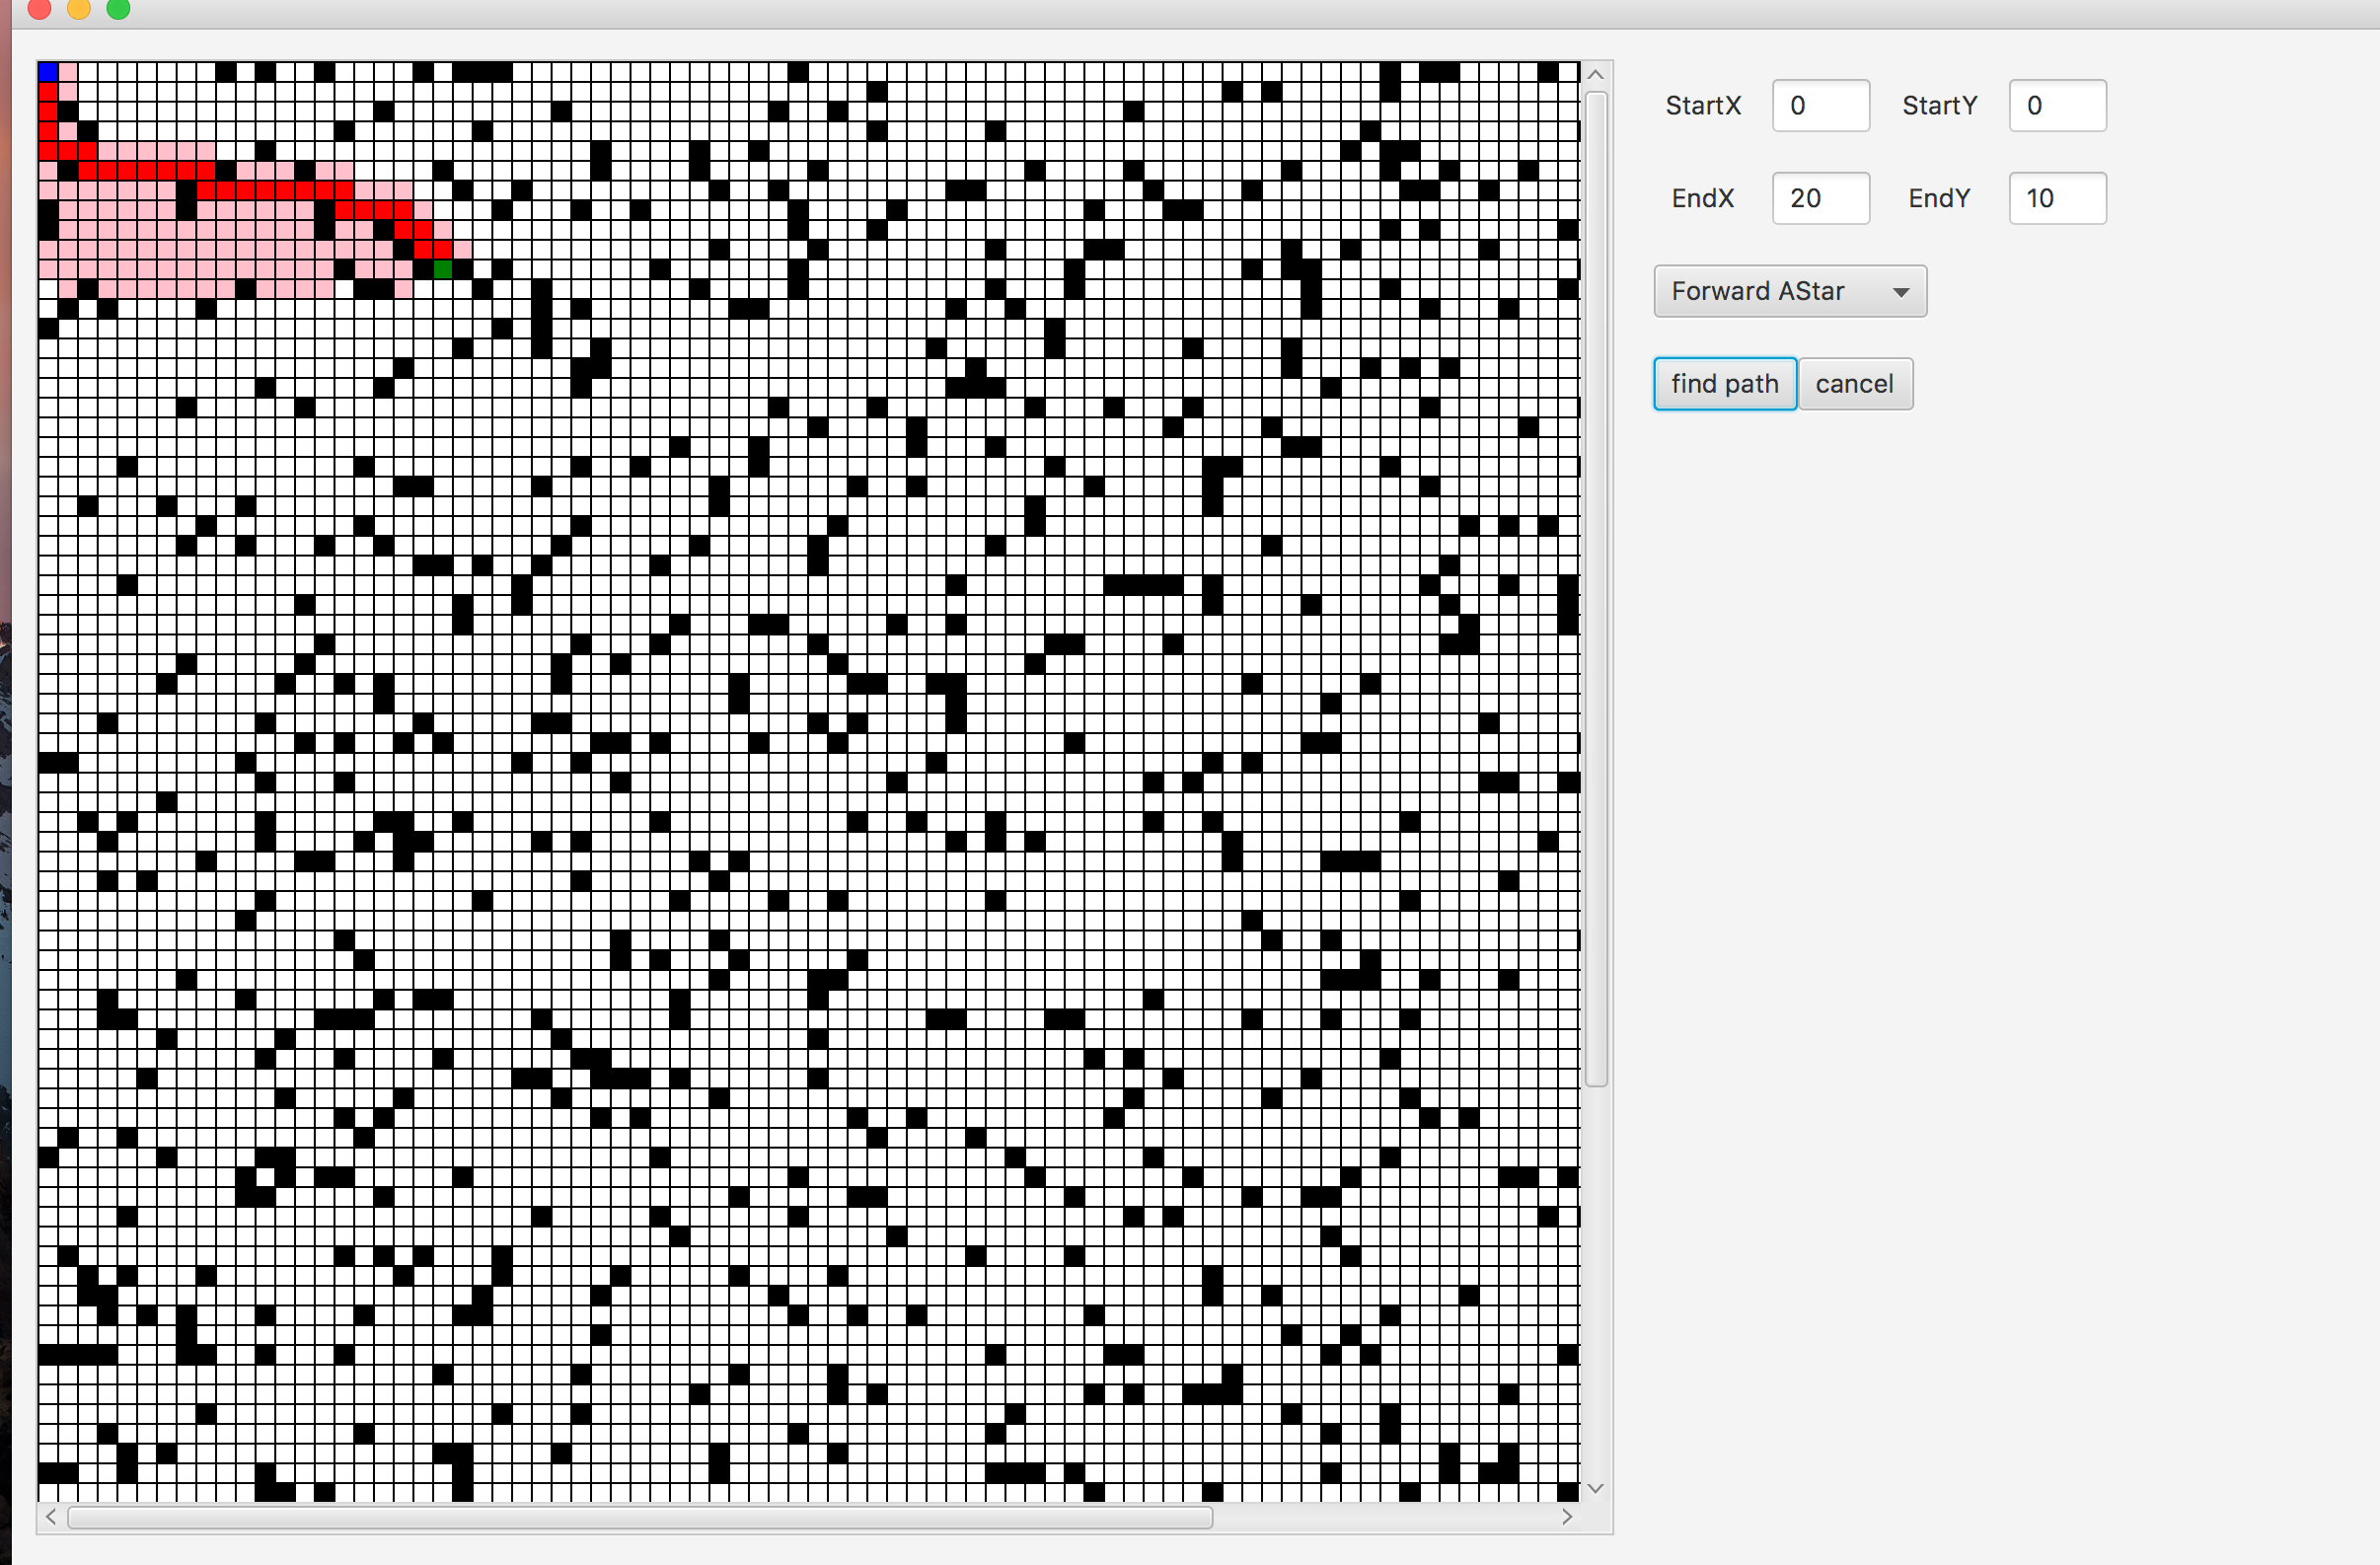
\includegraphics[width=1\linewidth,height=3in]{forward_a_star.png}

\subsection*{5.2}
Adaptive A*

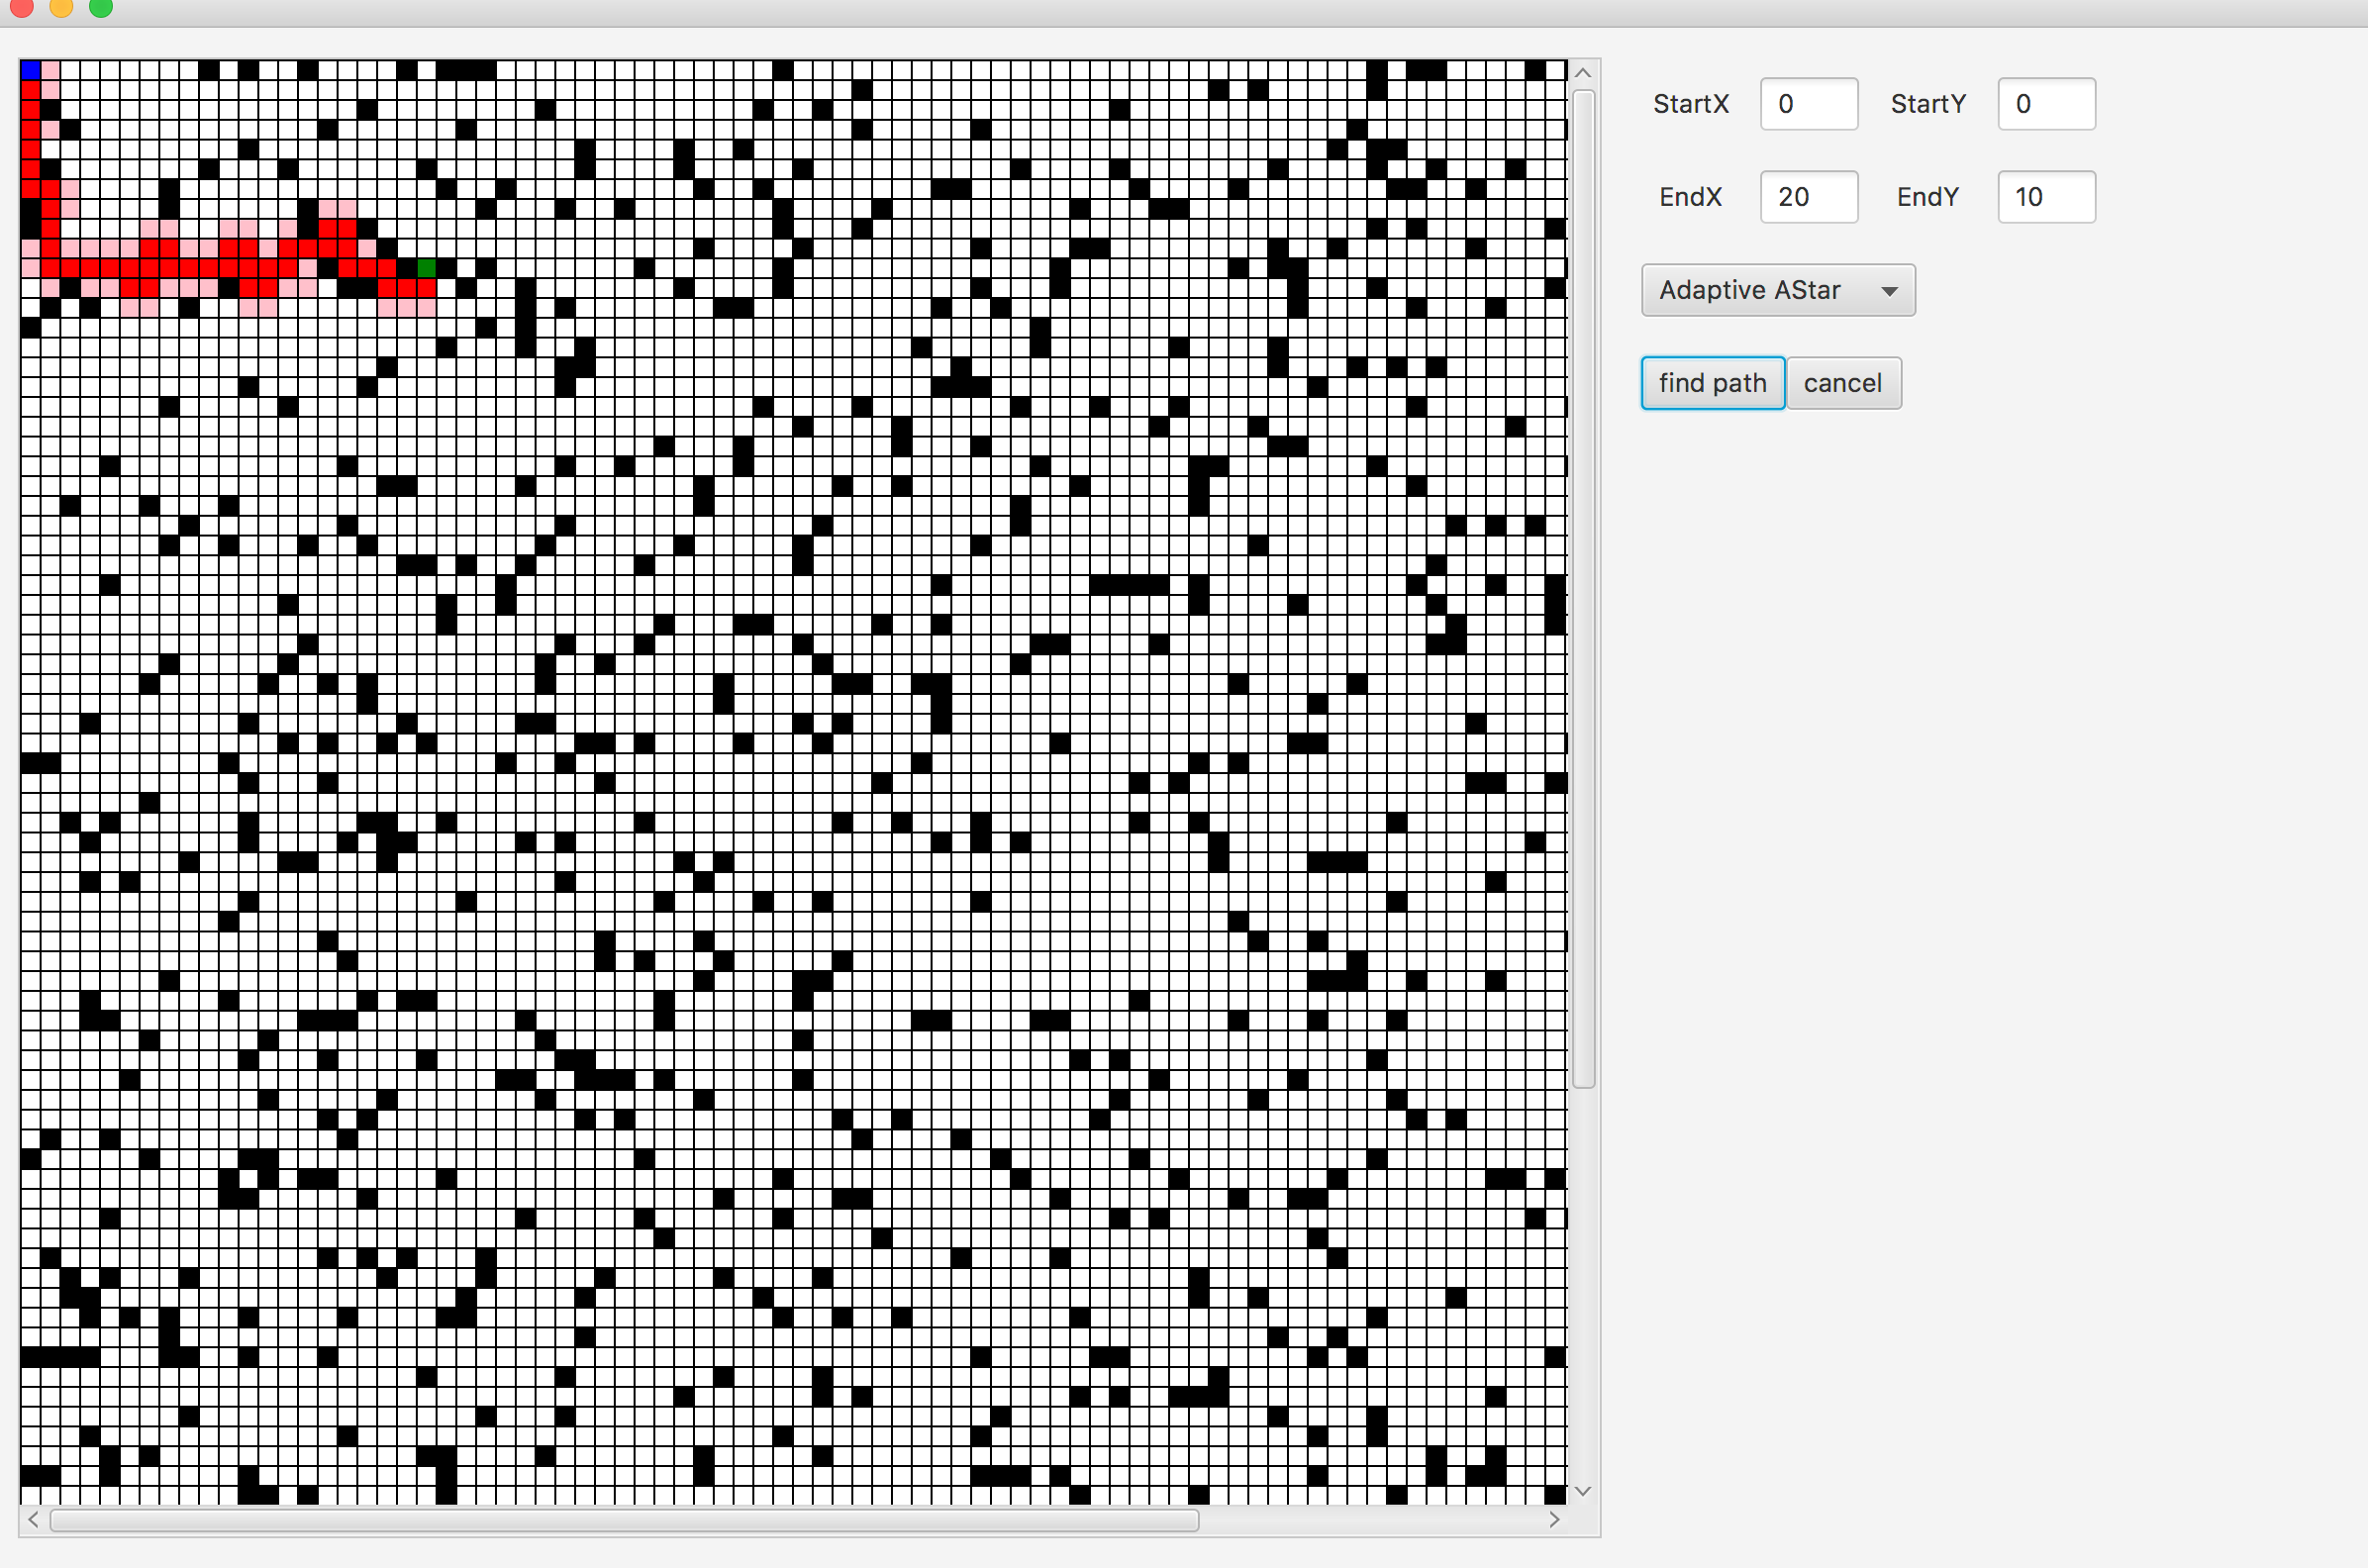
\includegraphics[width=1\linewidth,height=3in]{adaptive_a_star.png}

the results show that Adaptive A* expanded fewer cells than Repeated Forward A* and has less running time if the path is short enough. It is because
\newpage
\section*{Part 6}
The tree pointer can be represented as a two bit number .
\begin{lstlisting}
val directions = List((0, 1), (0, -1), (1, 0), (-1, 0))
\end{lstlisting}
It is calculated by father node coordinate minus child node coordinate.

Another way is to use sparse matrix representing the maze since the quantity of blocked cells is small enough.


\end{document}